\chapter{操作系统内核构建概述}
\section{什么是操作系统}
\subsection{体系结构}
如果我们站在一万米的高空来看 操作系统 ,可以发现操作系统这个系统软件干的事主要有两件:一是向下管理并控制计算机硬件和各种外设,二是向上管理应用软件并提供各种服务。我们可对其进一步定义为:操作系统是一种系统软件,主要功能是向下管理CPU、内存和各种外设等硬件资源,并形成软件执行环境来向上管理和服务应用软件。这样的描述也符合大多数操作系统教材上对操作系统的定义。为了完成这些工作,操作系统需要知道如何与硬件打交道,如何给应用软件提供服务。这就有一系列与操作系统相关的理论、抽象、设计等来支持如何做和做得好这两件事情。
\begin{figure}[htb]
	\centering
	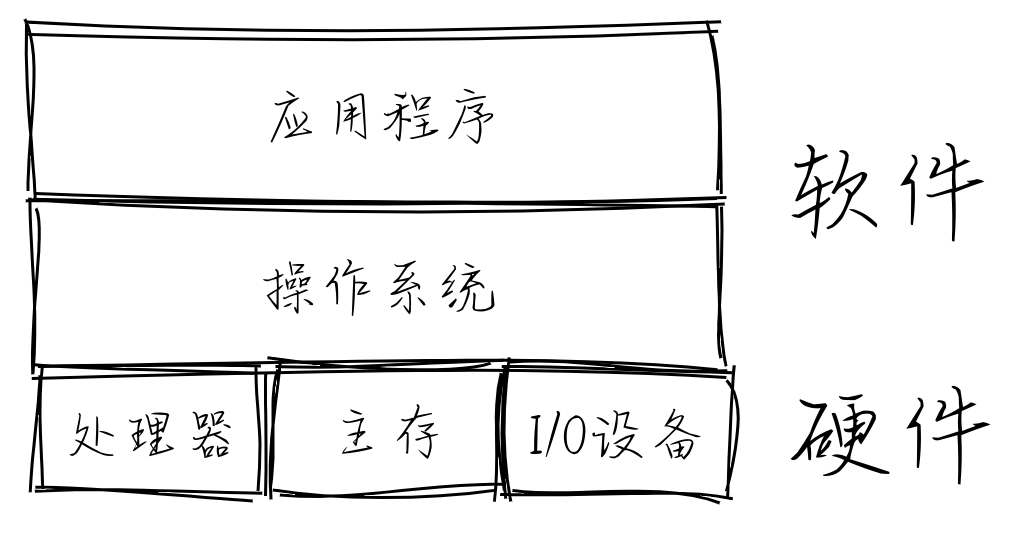
\includegraphics[width=\textwidth]{figures/01-01-computer-hw-sw.png}
	\caption{
		computer-hw-sw
	}
	\label{fig:computer-hw-sw}
\end{figure}
如果看看我们的身边, Android 应用运行在 ARM 处理器上的 Android 操作系统执行环境中;微软的 Office 应用运行在 x86-64 处理器上的 Windows 操作系统执行环境中;Web Server应用运行在 x86-64 处理器上的 Linux 操作系统执行环境中;Web app 应用运行在 x86-64 或 ARM 处理器上的 Chrome OS 操作系统执行环境中。而在一些嵌入式环境中,操作系统以运行时库的形式与应用程序紧密结合在一起,形成一个可在嵌入式硬件上执行的嵌入式应用。所以,在不同的应用场景下,操作系统的边界也是不同的,我们可以把运行时库、图形界面支持库等这些可支持不同应用的系统软件 (System Software) 也看成是操作系统的一部分。

那操作系统的组成部分包含哪些内容呢?在一般情况下,操作系统的主要组成包括:

\textbf{1、操作系统内核:}操作系统的核心部分,负责控制计算机的硬件资源并为用户和应用程序提供服务。

\textbf{2、系统工具和软件库:}为操作系统提供基本功能的软件,包括工具软件和系统软件库等。

\textbf{3、用户接口:}是操作系统的外壳,是用户与操作系统交互的方式。用户接口包括图形用户界面(GUI)和命令行界面(CLI)等。

而本书重点讲述的对象是操作系统内核,它的主要组成部分包括:

进程/线程管理:内核负责管理系统中的进程或线程,创建、销毁、调度和切换进程或线程。

内存管理:内核负责管理系统的内存,分配和回收内存空间,并保证进程之间的内存隔离。

文件系统:内核提供文件系统接口,负责管理存储设备上的文件和目录,并允许应用访问文件系统。

网络通信:内核提供网络通信接口,负责管理网络连接并允许应用进行网络通信。

设备驱动:内核提供设备驱动接口,负责管理硬件设备并允许应用和内核其他部分访问设备。

同步互斥:内核负责协调多个进程或线程之间对共享资源的访问。同步功能主要用于解决进程或线程之间的协作问题,互斥功能主要用于解决进程或线程之间的竞争问题。

系统调用接口:内核提供给应用程序访问系统服务的入口,应用程序通过系统调用接口调用操作系统提供的服务,如文件系统、网络通信、进程管理等。
\subsection{系统调用}
\textbf{什么是系统调用}
系统调用就是对操作系统内核中的一组用于实现系统功能的过程的调用。用户程序可以利用系统调用,向操作系统发出服务请求;操作系统通过系统调用为运行于其上的应用程序提供服务。
\textbf{API与ABI}
站在使用操作系统的角度会比较容易对操作系统内核的功能产生初步的认识。操作系统内核是一个提供各种服务的软件,其服务对象是应用程序,而用户(这里可以理解为一般使用计算机的人)是通过应用程序的服务间接获得操作系统的服务的,因此操作系统内核藏在一般用户看不到的地方。但应用程序需要访问操作系统获得操作系统的服务,这就需要通过操作系统的接口才能完成。操作系统与运行在用户态软件之间的接口形式就是应用程序二进制接口 (ABI, Application Binary Interface)。

操作系统不能只提供面向单一编程语言的函数库的编程接口 (API, Application Programming Interface) ,它的接口需要考虑对基于各种编程语言的应用支持,以及访问安全等因素,使得应用软件不能像访问函数库一样的直接访问操作系统内部函数,更不能直接读写操作系统内部的地址空间。为此,操作系统设计了一套安全可靠的二进制接口,我们称为系统调用接口 (System Call Interface)。系统调用接口通常面向应用程序提供了 API 的描述,但在具体实现上,还需要提供 ABI 的接口描述规范。

在现代处理器的安全支持(特权级隔离,内存空间隔离等)下,应用程序就不能直接以函数调用的方式访问操作系统的函数,以及直接读写操作系统的数据变量。不同类型的应用程序可以通过符合操作系统规定的系统调用接口,发出系统调用请求,来获得操作系统的服务。操作系统提供完服务后,返回应用程序继续执行。

\subsection{进程和内存}
\textbf{进程}

站在应用程序自身的角度来看,进程 (Process) 的一个经典定义是一个正在运行的程序实例。当程序运行在操作系统中的时候,从程序的视角来看,它会产生一种“幻觉”:即该程序是整个计算机系统中当前运行的唯一的程序,能够独占使用处理器、内存和外设,而且程序中的代码和数据是系统内存中唯一的对象。

然而,这种“幻觉”是操作系统为了便于应用的开发且不损失安全性刻意为应用程序营造出来的,它具体表现为“进程”这个抽象概念。站在计算机系统和操作系统的角度来看,并不存在这种“幻觉”。事实上,在一段时间之内,往往会有多个程序同时或交替在操作系统上运行,因此程序并不能独占整个计算机系统。具体而言,进程是应用程序的一次执行过程。并且在这个执行过程中,由“操作系统”执行环境来管理程序执行过程中的 进程上下文 – 一种控制流上下文。这里的进程上下文是指程序在运行中的各种物理/虚拟资源(寄存器、可访问的内存区域、打开的文件、信号等)的内容,特别是与程序执行相关的具体内容:内存中的代码和数据,栈、堆、当前执行的指令位置(程序计数器的内容)、当前执行时刻的各个通用寄存器中的值等。

我们知道,处理器是计算机系统中的硬件资源。为了提高处理器的利用率,操作系统需要让处理器足够忙,即让不同的程序轮流占用处理器来运行。如果一个程序因某个事件而不能运行下去时,就通过进程上下文切换把处理器占用权转交给另一个可运行程序。进程上下文切换如下图所示:
\begin{figure}[htb]
	\centering
	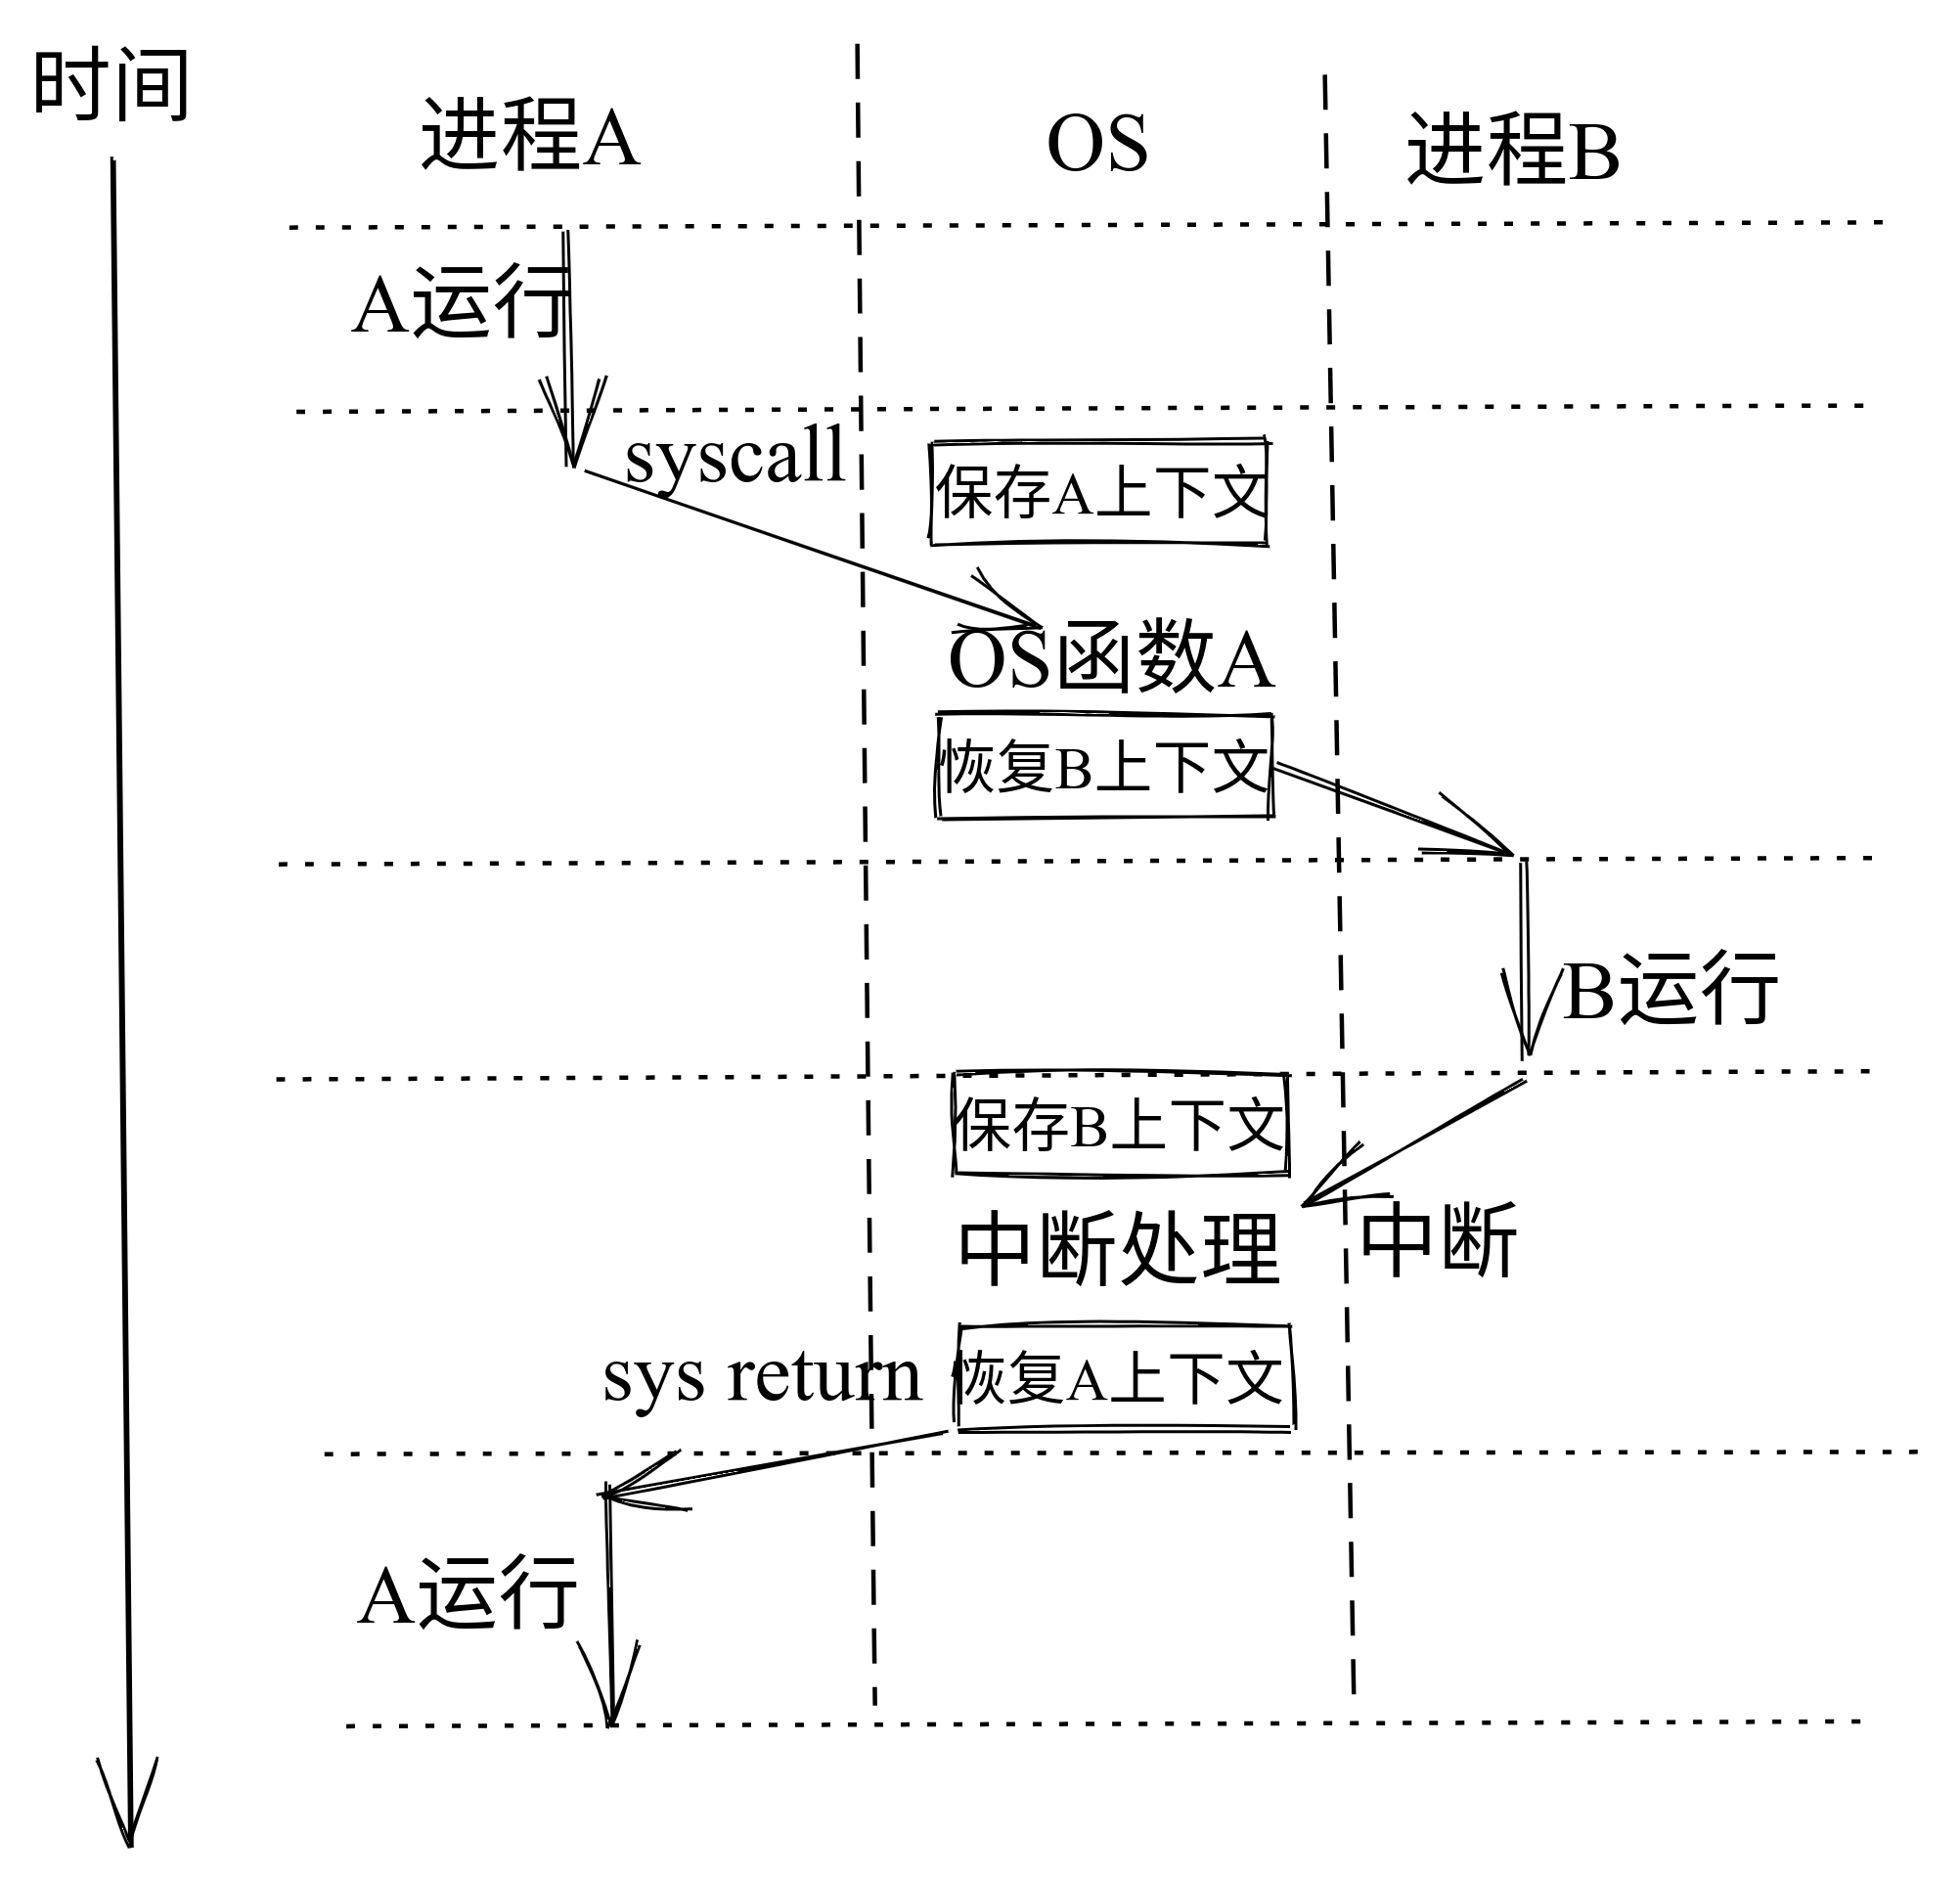
\includegraphics[width=\textwidth]{figures/02-01-context switch.png}
	\caption{
		context switch
	}
	\label{fig:context-switch}
\end{figure}

基于上面的介绍,我们可以给进程一个更加准确的定义:一个进程是一个具有一定独立功能的程序在一个数据集合上的一次动态执行过程。操作系统中的进程管理需要采用某种调度策略将处理器资源分配给程序并在适当的时候回收,并且要尽可能充分利用处理器的硬件资源。

\textbf{内存}
内存(Memory)是计算机的重要部件,也称内存储器和主存储器,它用于暂时存放CPU中的运算数据,以及与硬盘等外部存储器交换的数据。它是外存与CPU进行沟通的桥梁(缓和CPU和硬盘之间的速度矛盾),计算机中所有程序的运行都在内存中进行,内存性能的强弱影响计算机整体发挥的水平。只要计算机开始运行,操作系统就会把需要运算的数据从内存调到CPU中进行运算,当运算完成,CPU将结果传送出来。

内存管理,是指软件运行时对电脑内存资源的分配和使用的技术。其最主要的目的是如何高效、快速的分配,并且在适当的时候释放和回收内存资源。

一个执行中的程序,譬如网页浏览器在个人电脑或是图灵机(Turing machine)里面,为一个进程将资料转换于真实世界及电脑存储器之间,然后将资料存于电脑存储器内部(在电脑科学,一个程序是一群指令的集合,一个进程是电脑在执行中的程序)。存储器能被实际组织在许多方法里,例如磁带或是磁盘,或是小数组容量的微芯片。 从1950年代开始,电脑变的更复杂,它被连线于许多种类的存储器。内存管理的任务也变得复杂,甚至必须要在同一台机器上相同的时间执行多个进程。

在现代操作系统中,对于每个用户层(user-level)的程序,操作系统分配一段虚拟内存空间,当进程开始时,不需要加载磁盘中的用户程序到物理内存中,当用户真正使用到时,才会加载到物理内存中。

\subsection{I/O与文件系统}
\textbf{I/O设备}

在操作系统中,I/O设备的管理和控制非常重要。操作系统需要控制计算机的输入和输出,需要向设备发送命令,捕捉中断,并处理设备的各种错误,并为应用程序提供一个简单易用、统一的设备访问控制接口完成应用程序与设备的数据交互。同时,操作系统还需要控制设备的输入输出操作,保证数据的安全性和正确性。

I/O设备的操作通常需要使用一些系统调用来完成。这些系统调用是操作系统提供给应用程序的一组函数,用于进行输入输出操作。例如,系统调用read()可以用于从设备文件中读取数据,系统调用write()可以用于向设备文件中写入数据。

在操作系统的I/O管理中,通常会采用一些优化技术来提高设备的输入输出效率。例如,缓冲技术可以暂存一部分数据,减少直接对设备的读写次数;异步I/O技术可以允许应用程序在等待设备操作完成时继续执行其他任务;直接内存访问技术可以允许应用程序直接对内存进行读写操作,避免通过操作系统的缓冲区进行数据交换。

\textbf{文件系统}

文件系统是用于存储和组织文件的一种机制。文件系统通过特定的数据结构和算法,实现了对文件和目录的管理和控制,提供了方便的文件访问和使用方式。

文件系统的基本功能包括:存储信息、保存信息、共享信息(并发存取)。文件系统通过符号名来标识文件,便于用户使用;在多道程序系统中支持对文件的并发访问和控制;在不同的设备上提供同样的接口,方便用户操作和编程;同时,还提供多种文件访问权限,以及一定的差错恢复能力。

文件系统通过操作系统来进行管理,包括文件的结构、命名、存取、使用、保护和实现方法等。文件系统的架构通常包括设备驱动程序、基本文件系统等层次。设备驱动程序直接与外围设备通信,处理I/O请求的完成。基本文件系统又称为物理I/O层,是与计算机系统外部环境的基本接口。

文件系统中的文件是一组相似记录的集合,它被用户和应用程序视为一个实体,并可以通过名字访问。文件有一个唯一的文件名,可以被创建或删除。访问控制通常在文件级实施,也就是说,在一个共享系统中,用户和程序被允许或被拒绝访问整个文件。
